% Figure 1 — study workflow overview.
% Asset generated by scripts/publication_figures/fig01_workflow.py
\begin{figure}[tb]
  \centering
  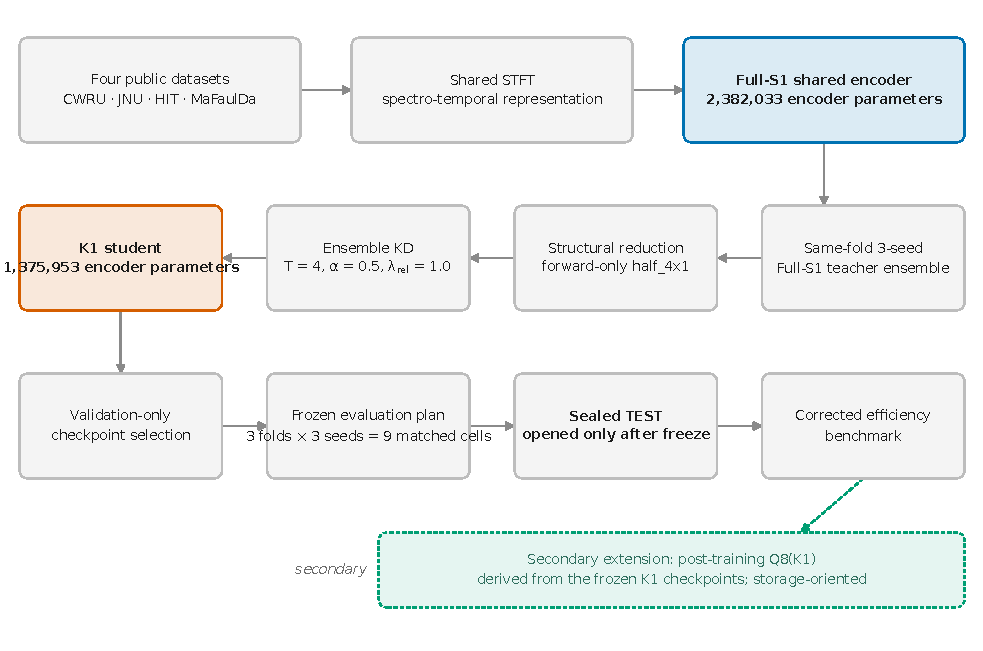
\includegraphics[width=\textwidth]{figures/fig01_workflow_overview.pdf}
  \caption{Overview of the frozen study workflow. One shared PC-STE encoder is
  trained across CWRU, JNU, HIT and MaFaulDa through a common spectro-temporal
  representation. The bidirectional Full-S1 encoder is structurally reduced to
  the forward-only K1 student, which is distilled from a same-fold ensemble of
  three independently seeded Full-S1 teachers. Checkpoints are selected on
  validation data only, and the sealed TEST partition was opened once, after the
  evaluation plan had been frozen. The post-training Q8(K1) stage (dashed) is a
  secondary, storage-oriented extension derived from the frozen K1 checkpoints
  and is not part of the primary comparison.}
  \label{fig:workflow}
\end{figure}
